\documentclass[twoside]{book}

% Packages required by doxygen
\usepackage{calc}
\usepackage{doxygen}
\usepackage{graphicx}
\usepackage[utf8]{inputenc}
\usepackage{makeidx}
\usepackage{multicol}
\usepackage{multirow}
\usepackage{textcomp}
\usepackage[table]{xcolor}

% Font selection
\usepackage[T1]{fontenc}
\usepackage{mathptmx}
\usepackage[scaled=.90]{helvet}
\usepackage{courier}
\usepackage{amssymb}
\usepackage{sectsty}
\renewcommand{\familydefault}{\sfdefault}
\allsectionsfont{%
  \fontseries{bc}\selectfont%
  \color{darkgray}%
}
\renewcommand{\DoxyLabelFont}{%
  \fontseries{bc}\selectfont%
  \color{darkgray}%
}

% Page & text layout
\usepackage{geometry}
\geometry{%
  a4paper,%
  top=2.5cm,%
  bottom=2.5cm,%
  left=2.5cm,%
  right=2.5cm%
}
\tolerance=750
\hfuzz=15pt
\hbadness=750
\setlength{\emergencystretch}{15pt}
\setlength{\parindent}{0cm}
\setlength{\parskip}{0.2cm}
\makeatletter
\renewcommand{\paragraph}{%
  \@startsection{paragraph}{4}{0ex}{-1.0ex}{1.0ex}{%
    \normalfont\normalsize\bfseries\SS@parafont%
  }%
}
\renewcommand{\subparagraph}{%
  \@startsection{subparagraph}{5}{0ex}{-1.0ex}{1.0ex}{%
    \normalfont\normalsize\bfseries\SS@subparafont%
  }%
}
\makeatother

% Headers & footers
\usepackage{fancyhdr}
\pagestyle{fancyplain}
\fancyhead[LE]{\fancyplain{}{\bfseries\thepage}}
\fancyhead[CE]{\fancyplain{}{}}
\fancyhead[RE]{\fancyplain{}{\bfseries\leftmark}}
\fancyhead[LO]{\fancyplain{}{\bfseries\rightmark}}
\fancyhead[CO]{\fancyplain{}{}}
\fancyhead[RO]{\fancyplain{}{\bfseries\thepage}}
\fancyfoot[LE]{\fancyplain{}{}}
\fancyfoot[CE]{\fancyplain{}{}}
\fancyfoot[RE]{\fancyplain{}{\bfseries\scriptsize Generated on Wed May 7 2014 18:45:30 for HE2mT Sensor Data Interface by Doxygen }}
\fancyfoot[LO]{\fancyplain{}{\bfseries\scriptsize Generated on Wed May 7 2014 18:45:30 for HE2mT Sensor Data Interface by Doxygen }}
\fancyfoot[CO]{\fancyplain{}{}}
\fancyfoot[RO]{\fancyplain{}{}}
\renewcommand{\footrulewidth}{0.4pt}
\renewcommand{\chaptermark}[1]{%
  \markboth{#1}{}%
}
\renewcommand{\sectionmark}[1]{%
  \markright{\thesection\ #1}%
}

% Indices & bibliography
\usepackage{natbib}
\usepackage[titles]{tocloft}
\setcounter{tocdepth}{3}
\setcounter{secnumdepth}{5}
\makeindex

% Hyperlinks (required, but should be loaded last)
\usepackage{ifpdf}
\ifpdf
  \usepackage[pdftex,pagebackref=true]{hyperref}
\else
  \usepackage[ps2pdf,pagebackref=true]{hyperref}
\fi
\hypersetup{%
  colorlinks=true,%
  linkcolor=blue,%
  citecolor=blue,%
  unicode%
}

% Custom commands
\newcommand{\clearemptydoublepage}{%
  \newpage{\pagestyle{empty}\cleardoublepage}%
}


%===== C O N T E N T S =====

\begin{document}

% Titlepage & ToC
\hypersetup{pageanchor=false}
\pagenumbering{roman}
\begin{titlepage}
\vspace*{7cm}
\begin{center}%
{\Large H\-E2m\-T Sensor Data Interface \\[1ex]\large 0.\-1 }\\
\vspace*{1cm}
{\large Generated by Doxygen 1.8.4}\\
\vspace*{0.5cm}
{\small Wed May 7 2014 18:45:30}\\
\end{center}
\end{titlepage}
\clearemptydoublepage
\tableofcontents
\clearemptydoublepage
\pagenumbering{arabic}
\hypersetup{pageanchor=true}

%--- Begin generated contents ---
\chapter{Main Page}
\label{index}\hypertarget{index}{}\hypertarget{index_secScope}{}\section{Scope}\label{index_secScope}
This interface must be implemented by an application server (A\-S) or replication framework (R\-F) to receive sensor data from a sensor aggregation system (S\-A\-S). In addition, it is used to pass on sensor data from the replication framework (R\-F) to the appserver (A\-S).  
\begin{DoxyImage}
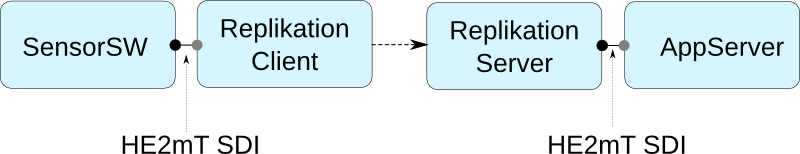
\includegraphics{interfaces.png}
\caption{width=1.0}
\end{DoxyImage}
\hypertarget{index_secGeneral}{}\section{General}\label{index_secGeneral}
All functions of this abstract class need to be implemented in order to receive sensor data. The functions of \hyperlink{classgeneric_param_interface}{generic\-Param\-Interface} need not be implemented. However, \hyperlink{classgeneric_param_interface}{generic\-Param\-Interface} can be used to expose a parameter interface that allows the sensor aggregation system to modify certain values of the application server. It is for debugging purposes, only. On java, \hyperlink{classgeneric_param_interface}{generic\-Param\-Interface} needs not to be implemented.

The interface is used as follows\-:
\begin{DoxyItemize}
\item First, the application using it calls \hyperlink{classhe2mt_s_d_i_a6a3b5da850e0571bc4a8c8e0de7ad9e8}{he2mt\-S\-D\-I\-::init()}
\item Then, it calls \hyperlink{classhe2mt_s_d_i_ae5212f96e535b795b11fd34a89a3d616}{he2mt\-S\-D\-I\-::authorize()}, providing authentication/authorization credentials. If no authentication/authorization is needed, the class implementing the interface can safely ignore all paramters and do nothing.\par

\item Then, data can be transferred via the interface by calling he2mt\-S\-D\-I\-::set\-Data()
\end{DoxyItemize}

When everything is done, the application can call \hyperlink{classhe2mt_s_d_i_a7f9d573e91544cc1436dab6bf1a889cf}{he2mt\-S\-D\-I\-::disconnect()} to stop being authenticated.\hypertarget{index_secSlots}{}\section{Data Slots}\label{index_secSlots}
The interface defines data slots. Data slots are virtual channels that an application can read from or write to. The interface is unidirectional, meaning a class implementing the interface can only read from a data slot (by implementing set\-Sensor\-Data), whereas the application using it (S\-A\-S or R\-F) can write to this data slot by calling \hyperlink{classhe2mt_s_d_i_a775fcd2c08e923050b76aa750895a983}{he2mt\-S\-D\-I\-::set\-Sensor\-Data()}. read more\-: \hyperlink{he2mt_s_d_i_data_slots_8h}{he2mt\-S\-D\-I\-Data\-Slots.\-h} \hypertarget{index_secSample}{}\section{Sample Program}\label{index_secSample}
The following code would use the interface correctly\-:

\#include \char`\"{}implementations/he2mt\-S\-D\-I\-Rest.\-hpp\char`\"{} \par
 int main()\{\par
 float values\mbox{[}6\mbox{]} = \{1,2,3,4,5,6\};\par
 uint32\-\_\-t activity = H\-E2\-M\-T\-\_\-\-S\-D\-I\-\_\-\-D\-A\-T\-A\-\_\-\-S\-L\-O\-T\-\_\-\-A\-C\-T\-I\-V\-I\-T\-Y\-\_\-\-V\-A\-L\-U\-E\-\_\-\-W\-A\-L\-K\-I\-N\-G;\par
 he2mt\-S\-D\-I\-Rest r;\par
 r.\-init();\par
 if(r.\-authorize(\char`\"{}id\char`\"{},\char`\"{}secret\char`\"{},\char`\"{}he2mt\-\_\-user\char`\"{},\char`\"{}he2mt\-\_\-user\char`\"{}))\{\par
 r.\-set\-Sensor\-Data(H\-E2\-M\-T\-\_\-\-S\-D\-I\-\_\-\-D\-A\-T\-A\-\_\-\-S\-L\-O\-T\-\_\-\-A\-C\-T\-I\-V\-I\-T\-Y,\char`\"{}0\char`\"{},\char`\"{}0\char`\"{},0.\-01,1,\&activity);\par
 r.\-set\-Sensor\-Data(H\-E2\-M\-T\-\_\-\-S\-D\-I\-\_\-\-D\-A\-T\-A\-\_\-\-S\-L\-O\-T\-\_\-\-R\-A\-W\-A\-C\-C,\char`\"{}0\char`\"{},\char`\"{}0\char`\"{},0.\-01,2,\&values);\par
 \}\par
 r.\-disconnect();\par
 \}\par
 
\chapter{Hierarchical Index}
\section{Class Hierarchy}
This inheritance list is sorted roughly, but not completely, alphabetically\-:\begin{DoxyCompactList}
\item \contentsline{section}{generic\-Param\-Interface}{\pageref{classgeneric_param_interface}}{}
\begin{DoxyCompactList}
\item \contentsline{section}{he2mt\-S\-D\-I}{\pageref{classhe2mt_s_d_i}}{}
\end{DoxyCompactList}
\end{DoxyCompactList}

\chapter{Class Index}
\section{Class List}
Here are the classes, structs, unions and interfaces with brief descriptions\-:\begin{DoxyCompactList}
\item\contentsline{section}{\hyperlink{classgeneric_param_interface}{generic\-Param\-Interface} \\*Class that allows the exchange of parameter values in a generic way }{\pageref{classgeneric_param_interface}}{}
\item\contentsline{section}{\hyperlink{classhe2mt_s_d_i}{he2mt\-S\-D\-I} \\*Purely virtual (abstract) class that needs to be implemented to get sensor data via the H\-E2m\-T S\-D\-I The class \char`\"{}generic\-Param\-Interface\char`\"{} is for debugging purposes, only. It is not part of the interface. The standard C++ installation comes with a dummy implementation of \hyperlink{classgeneric_param_interface}{generic\-Param\-Interface} as the accsensor\-\_\-server -\/ application expects it to be there. In Java on a mobile phone, \hyperlink{classgeneric_param_interface}{generic\-Param\-Interface} needs not to be implemented at all }{\pageref{classhe2mt_s_d_i}}{}
\end{DoxyCompactList}

\chapter{File Index}
\section{File List}
Here is a list of all documented files with brief descriptions\-:\begin{DoxyCompactList}
\item\contentsline{section}{/home/kindt/workspace/\-H\-E2m\-T/projects/libs/he2mt\-S\-D\-I/src/\hyperlink{generic_param_interface_8h}{generic\-Param\-Interface.\-h} \\*A generic interface to exchange parameters with a class derived from it }{\pageref{generic_param_interface_8h}}{}
\item\contentsline{section}{/home/kindt/workspace/\-H\-E2m\-T/projects/libs/he2mt\-S\-D\-I/src/\hyperlink{he2mt_debug_8h}{he2mt\-Debug.\-h} }{\pageref{he2mt_debug_8h}}{}
\item\contentsline{section}{/home/kindt/workspace/\-H\-E2m\-T/projects/libs/he2mt\-S\-D\-I/src/\hyperlink{he2mt_s_d_i_8hpp}{he2mt\-S\-D\-I.\-hpp} \\*He2m\-T interface class for all sensors to the replication -\/ and/or application server interface }{\pageref{he2mt_s_d_i_8hpp}}{}
\item\contentsline{section}{/home/kindt/workspace/\-H\-E2m\-T/projects/libs/he2mt\-S\-D\-I/src/\hyperlink{he2mt_s_d_i_data_slots_8h}{he2mt\-S\-D\-I\-Data\-Slots.\-h} \\*Data slot definitions for H\-E2m\-T S\-D\-I }{\pageref{he2mt_s_d_i_data_slots_8h}}{}
\item\contentsline{section}{/home/kindt/workspace/\-H\-E2m\-T/projects/libs/he2mt\-S\-D\-I/src/\hyperlink{he2mt_s_d_i_error_codes_8h}{he2mt\-S\-D\-I\-Error\-Codes.\-h} \\*Error Code defintions for H\-E2m\-T S\-D\-I }{\pageref{he2mt_s_d_i_error_codes_8h}}{}
\end{DoxyCompactList}

\chapter{Class Documentation}
\hypertarget{classgeneric_param_interface}{\section{generic\-Param\-Interface Class Reference}
\label{classgeneric_param_interface}\index{generic\-Param\-Interface@{generic\-Param\-Interface}}
}


Class that allows the exchange of parameter values in a generic way.  




{\ttfamily \#include $<$generic\-Param\-Interface.\-h$>$}

Inheritance diagram for generic\-Param\-Interface\-:\begin{figure}[H]
\begin{center}
\leavevmode
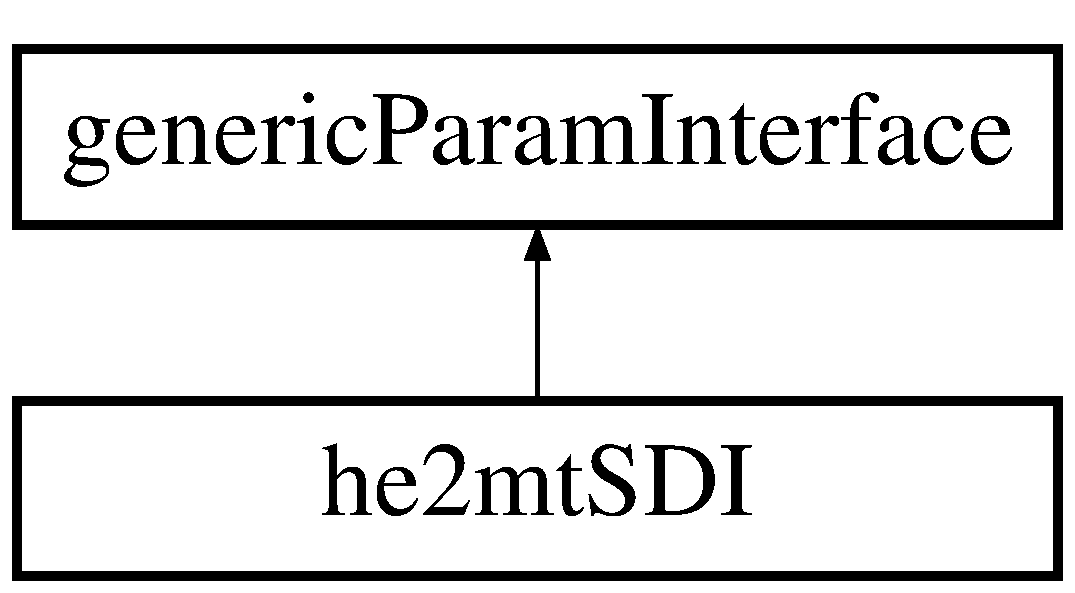
\includegraphics[height=2.000000cm]{classgeneric_param_interface}
\end{center}
\end{figure}
\subsection*{Public Member Functions}
\begin{DoxyCompactItemize}
\item 
virtual bool \hyperlink{classgeneric_param_interface_a8d3d4123db419e649fe73adf4b498135}{get\-Param} (const char $\ast$ident, char $\ast$value)
\begin{DoxyCompactList}\small\item\em Read out a param. Read out a param. \end{DoxyCompactList}\item 
virtual bool \hyperlink{classgeneric_param_interface_aeb0cf7b216209f4514f5285c3d57f5fd}{set\-Param} (const char $\ast$ident, const char $\ast$value)
\begin{DoxyCompactList}\small\item\em Set param \char`\"{}ident\char`\"{} to value \char`\"{}value\char`\"{}. \end{DoxyCompactList}\item 
virtual char $\ast$ \hyperlink{classgeneric_param_interface_a10302cc5d418fff17ff222c2d74fc13d}{get\-Param\-List} ()
\begin{DoxyCompactList}\small\item\em Generates a machine-\/readable list of all parameters available param List format (E\-B\-N\-F)\-: Ascii string that is fomratted like follows. param\-List = \{param\-Line\}\par
 param\-Line = ident \char`\"{}$|$\char`\"{} decident \char`\"{}$|$\char`\"{} limit\-Min \char`\"{}$|$\char`\"{} limit\-Max \char`\"{}\textbackslash{}n\char`\"{}\par
 ident \-: string identifiing the param, must be compatible with the first param of \hyperlink{classgeneric_param_interface_a8d3d4123db419e649fe73adf4b498135}{get\-Param()};\par
 decident \-: decident. The first character identifies the value type of the param. Possible values\-:\par
 \char`\"{}f\char`\"{}\-: float\par
 \char`\"{}d\char`\"{}\-: decimal\par
 \char`\"{}s\char`\"{}\-: string\par
 in case of floats, \char`\"{}f\char`\"{} ma be follwoed by the number of decimals. Example\-: \char`\"{}f11\char`\"{} =$>$ 11 decimals precision\par
 limit\-Min \-:floating point number specifyng the minimal value of the param. ignored for strings\par
 limit\-Max \-:floating point number specifying the maximal value of the param. For strings, if 0, the string can have abitrary lenght. Other wise, the max lenght will be set to this value\par
 \end{DoxyCompactList}\item 
virtual void \hyperlink{classgeneric_param_interface_af210b50a000af4466a17dff15c84bd4a}{get\-Ident} (char $\ast$ident)
\begin{DoxyCompactList}\small\item\em Provides a string containing an identifier (i.\-e. Name) of the class that implements the \hyperlink{classgeneric_param_interface}{generic\-Param\-Interface}. \end{DoxyCompactList}\end{DoxyCompactItemize}


\subsection{Detailed Description}
Class that allows the exchange of parameter values in a generic way. 

\subsection{Member Function Documentation}
\hypertarget{classgeneric_param_interface_af210b50a000af4466a17dff15c84bd4a}{\index{generic\-Param\-Interface@{generic\-Param\-Interface}!get\-Ident@{get\-Ident}}
\index{get\-Ident@{get\-Ident}!genericParamInterface@{generic\-Param\-Interface}}
\subsubsection[{get\-Ident}]{\setlength{\rightskip}{0pt plus 5cm}virtual void generic\-Param\-Interface\-::get\-Ident (
\begin{DoxyParamCaption}
\item[{char $\ast$}]{ident}
\end{DoxyParamCaption}
)\hspace{0.3cm}{\ttfamily [inline]}, {\ttfamily [virtual]}}}\label{classgeneric_param_interface_af210b50a000af4466a17dff15c84bd4a}


Provides a string containing an identifier (i.\-e. Name) of the class that implements the \hyperlink{classgeneric_param_interface}{generic\-Param\-Interface}. 


\begin{DoxyParams}{Parameters}
{\em ident} & Non-\/empty, writable buffer of at least 256 bytes of space to write the name into. \\
\hline
\end{DoxyParams}
\hypertarget{classgeneric_param_interface_a8d3d4123db419e649fe73adf4b498135}{\index{generic\-Param\-Interface@{generic\-Param\-Interface}!get\-Param@{get\-Param}}
\index{get\-Param@{get\-Param}!genericParamInterface@{generic\-Param\-Interface}}
\subsubsection[{get\-Param}]{\setlength{\rightskip}{0pt plus 5cm}virtual bool generic\-Param\-Interface\-::get\-Param (
\begin{DoxyParamCaption}
\item[{const char $\ast$}]{ident, }
\item[{char $\ast$}]{value}
\end{DoxyParamCaption}
)\hspace{0.3cm}{\ttfamily [inline]}, {\ttfamily [virtual]}}}\label{classgeneric_param_interface_a8d3d4123db419e649fe73adf4b498135}


Read out a param. Read out a param. 


\begin{DoxyParams}{Parameters}
{\em ident} & Paremter identification string. Memory management is to be done by the caller. \\
\hline
{\em value} & A writable, empty buffer to be filled by the called function. Memory management is to be done by the caller. At least 256 bytes of buffer need to be provided \\
\hline
\end{DoxyParams}
\begin{DoxyReturn}{Returns}
true if successful, false, if not 
\end{DoxyReturn}
\hypertarget{classgeneric_param_interface_a10302cc5d418fff17ff222c2d74fc13d}{\index{generic\-Param\-Interface@{generic\-Param\-Interface}!get\-Param\-List@{get\-Param\-List}}
\index{get\-Param\-List@{get\-Param\-List}!genericParamInterface@{generic\-Param\-Interface}}
\subsubsection[{get\-Param\-List}]{\setlength{\rightskip}{0pt plus 5cm}virtual char$\ast$ generic\-Param\-Interface\-::get\-Param\-List (
\begin{DoxyParamCaption}
{}
\end{DoxyParamCaption}
)\hspace{0.3cm}{\ttfamily [inline]}, {\ttfamily [virtual]}}}\label{classgeneric_param_interface_a10302cc5d418fff17ff222c2d74fc13d}


Generates a machine-\/readable list of all parameters available param List format (E\-B\-N\-F)\-: Ascii string that is fomratted like follows. param\-List = \{param\-Line\}\par
 param\-Line = ident \char`\"{}$|$\char`\"{} decident \char`\"{}$|$\char`\"{} limit\-Min \char`\"{}$|$\char`\"{} limit\-Max \char`\"{}\textbackslash{}n\char`\"{}\par
 ident \-: string identifiing the param, must be compatible with the first param of \hyperlink{classgeneric_param_interface_a8d3d4123db419e649fe73adf4b498135}{get\-Param()};\par
 decident \-: decident. The first character identifies the value type of the param. Possible values\-:\par
 \char`\"{}f\char`\"{}\-: float\par
 \char`\"{}d\char`\"{}\-: decimal\par
 \char`\"{}s\char`\"{}\-: string\par
 in case of floats, \char`\"{}f\char`\"{} ma be follwoed by the number of decimals. Example\-: \char`\"{}f11\char`\"{} =$>$ 11 decimals precision\par
 limit\-Min \-:floating point number specifyng the minimal value of the param. ignored for strings\par
 limit\-Max \-:floating point number specifying the maximal value of the param. For strings, if 0, the string can have abitrary lenght. Other wise, the max lenght will be set to this value\par
 

\begin{DoxyReturn}{Returns}
String containing the parameter list. It will be alloc'ed by the function using malloc() and should be free'd after use using free() 
\end{DoxyReturn}
\hypertarget{classgeneric_param_interface_aeb0cf7b216209f4514f5285c3d57f5fd}{\index{generic\-Param\-Interface@{generic\-Param\-Interface}!set\-Param@{set\-Param}}
\index{set\-Param@{set\-Param}!genericParamInterface@{generic\-Param\-Interface}}
\subsubsection[{set\-Param}]{\setlength{\rightskip}{0pt plus 5cm}virtual bool generic\-Param\-Interface\-::set\-Param (
\begin{DoxyParamCaption}
\item[{const char $\ast$}]{ident, }
\item[{const char $\ast$}]{value}
\end{DoxyParamCaption}
)\hspace{0.3cm}{\ttfamily [inline]}, {\ttfamily [virtual]}}}\label{classgeneric_param_interface_aeb0cf7b216209f4514f5285c3d57f5fd}


Set param \char`\"{}ident\char`\"{} to value \char`\"{}value\char`\"{}. 


\begin{DoxyParams}{Parameters}
{\em ident} & Paremter identification string. Memory management is to be done by the caller. \\
\hline
{\em value} & A buffer containing the value to be set. Memory management is to be done by the caller. \\
\hline
\end{DoxyParams}
\begin{DoxyReturn}{Returns}

\end{DoxyReturn}


The documentation for this class was generated from the following file\-:\begin{DoxyCompactItemize}
\item 
/home/kindt/workspace/\-H\-E2m\-T/projects/libs/he2mt\-S\-D\-I/src/\hyperlink{generic_param_interface_8h}{generic\-Param\-Interface.\-h}\end{DoxyCompactItemize}

\hypertarget{classhe2mt_s_d_i}{\section{he2mt\-S\-D\-I Class Reference}
\label{classhe2mt_s_d_i}\index{he2mt\-S\-D\-I@{he2mt\-S\-D\-I}}
}


Purely virtual (abstract) class that needs to be implemented to get sensor data via the H\-E2m\-T S\-D\-I The class \char`\"{}generic\-Param\-Interface\char`\"{} is for debugging purposes, only. It is not part of the interface. The standard C++ installation comes with a dummy implementation of \hyperlink{classgeneric_param_interface}{generic\-Param\-Interface} as the accsensor\-\_\-server -\/ application expects it to be there. In Java on a mobile phone, \hyperlink{classgeneric_param_interface}{generic\-Param\-Interface} needs not to be implemented at all.  




{\ttfamily \#include $<$he2mt\-S\-D\-I.\-hpp$>$}

Inheritance diagram for he2mt\-S\-D\-I\-:\begin{figure}[H]
\begin{center}
\leavevmode
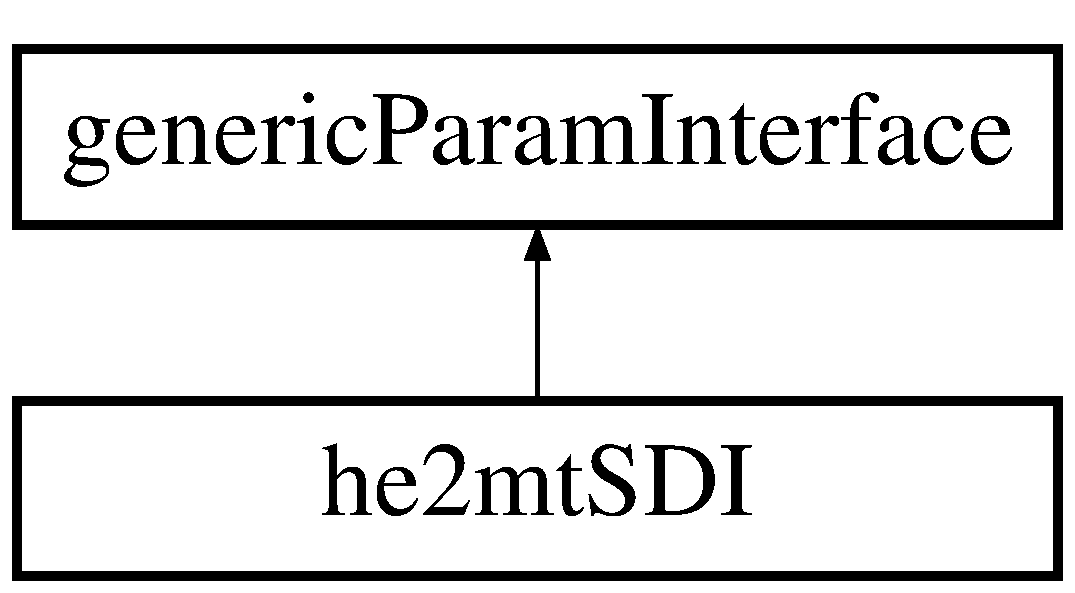
\includegraphics[height=2.000000cm]{classhe2mt_s_d_i}
\end{center}
\end{figure}
\subsection*{Public Types}
\begin{DoxyCompactItemize}
\item 
typedef uint32\-\_\-t \hyperlink{classhe2mt_s_d_i_ad0bd9136f18c52d27b93cfca85bf05dd}{dataslot\-\_\-t}
\item 
typedef uint32\-\_\-t \hyperlink{classhe2mt_s_d_i_aa527ccf96fd5eacc154c1c23e56fc9fd}{errorcode\-\_\-t}
\end{DoxyCompactItemize}
\subsection*{Public Member Functions}
\begin{DoxyCompactItemize}
\item 
\hypertarget{classhe2mt_s_d_i_a6a3b5da850e0571bc4a8c8e0de7ad9e8}{virtual void \hyperlink{classhe2mt_s_d_i_a6a3b5da850e0571bc4a8c8e0de7ad9e8}{init} ()=0}\label{classhe2mt_s_d_i_a6a3b5da850e0571bc4a8c8e0de7ad9e8}

\begin{DoxyCompactList}\small\item\em Initialization function. This function will be called once before any other function is called. \end{DoxyCompactList}\item 
virtual bool \hyperlink{classhe2mt_s_d_i_ae5212f96e535b795b11fd34a89a3d616}{authorize} (char $\ast$application\-I\-D, char $\ast$application\-Secret, char $\ast$username, char $\ast$password)=0
\begin{DoxyCompactList}\small\item\em authorize sensor aggregation system against remote side This function authorizes the sensor aggregation system against the replication framework and/or appserver. It is oauth-\/compatible. \end{DoxyCompactList}\item 
virtual bool \hyperlink{classhe2mt_s_d_i_a775fcd2c08e923050b76aa750895a983}{set\-Sensor\-Data} (\hyperlink{classhe2mt_s_d_i_ad0bd9136f18c52d27b93cfca85bf05dd}{dataslot\-\_\-t} data\-Slot, char $\ast$sensor\-Address, char $\ast$time\-Stamp\-Sensor, double sampling\-Period, uint32\-\_\-t n\-Values, void $\ast$value\-List)=0
\begin{DoxyCompactList}\small\item\em write new sensor data This function is called whenever sensor data \end{DoxyCompactList}\item 
virtual bool \hyperlink{classhe2mt_s_d_i_a7f9d573e91544cc1436dab6bf1a889cf}{disconnect} ()=0
\begin{DoxyCompactList}\small\item\em disconnect S\-A\-S from the A\-S/\-R\-F. This function is called when the sensor interface wishes to unregister with the A\-S/\-R\-F. The expected behaviour is that the authorization is invalidated. \end{DoxyCompactList}\item 
virtual \hyperlink{classhe2mt_s_d_i_aa527ccf96fd5eacc154c1c23e56fc9fd}{errorcode\-\_\-t} \hyperlink{classhe2mt_s_d_i_a2f0bf651098d94ab7ffc04f7b3b00fdf}{get\-Last\-Error} ()=0
\begin{DoxyCompactList}\small\item\em Get the number of the last error that has occurred. The error numbers are defined by the interface and are similar for all implementations of this interface. \end{DoxyCompactList}\item 
virtual void $\ast$ \hyperlink{classhe2mt_s_d_i_ab95b4854cfc4841a7f2dae073fa011fe}{get\-Application\-Error\-Info} ()=0
\begin{DoxyCompactList}\small\item\em Get implementation-\/specific information ont the error. \end{DoxyCompactList}\end{DoxyCompactItemize}


\subsection{Detailed Description}
Purely virtual (abstract) class that needs to be implemented to get sensor data via the H\-E2m\-T S\-D\-I The class \char`\"{}generic\-Param\-Interface\char`\"{} is for debugging purposes, only. It is not part of the interface. The standard C++ installation comes with a dummy implementation of \hyperlink{classgeneric_param_interface}{generic\-Param\-Interface} as the accsensor\-\_\-server -\/ application expects it to be there. In Java on a mobile phone, \hyperlink{classgeneric_param_interface}{generic\-Param\-Interface} needs not to be implemented at all. 

\subsection{Member Typedef Documentation}
\hypertarget{classhe2mt_s_d_i_ad0bd9136f18c52d27b93cfca85bf05dd}{\index{he2mt\-S\-D\-I@{he2mt\-S\-D\-I}!dataslot\-\_\-t@{dataslot\-\_\-t}}
\index{dataslot\-\_\-t@{dataslot\-\_\-t}!he2mtSDI@{he2mt\-S\-D\-I}}
\subsubsection[{dataslot\-\_\-t}]{\setlength{\rightskip}{0pt plus 5cm}typedef uint32\-\_\-t {\bf he2mt\-S\-D\-I\-::dataslot\-\_\-t}}}\label{classhe2mt_s_d_i_ad0bd9136f18c52d27b93cfca85bf05dd}
Data type for the data slot numbers \hypertarget{classhe2mt_s_d_i_aa527ccf96fd5eacc154c1c23e56fc9fd}{\index{he2mt\-S\-D\-I@{he2mt\-S\-D\-I}!errorcode\-\_\-t@{errorcode\-\_\-t}}
\index{errorcode\-\_\-t@{errorcode\-\_\-t}!he2mtSDI@{he2mt\-S\-D\-I}}
\subsubsection[{errorcode\-\_\-t}]{\setlength{\rightskip}{0pt plus 5cm}typedef uint32\-\_\-t {\bf he2mt\-S\-D\-I\-::errorcode\-\_\-t}}}\label{classhe2mt_s_d_i_aa527ccf96fd5eacc154c1c23e56fc9fd}
Data type for the error codes 

\subsection{Member Function Documentation}
\hypertarget{classhe2mt_s_d_i_ae5212f96e535b795b11fd34a89a3d616}{\index{he2mt\-S\-D\-I@{he2mt\-S\-D\-I}!authorize@{authorize}}
\index{authorize@{authorize}!he2mtSDI@{he2mt\-S\-D\-I}}
\subsubsection[{authorize}]{\setlength{\rightskip}{0pt plus 5cm}virtual bool he2mt\-S\-D\-I\-::authorize (
\begin{DoxyParamCaption}
\item[{char $\ast$}]{application\-I\-D, }
\item[{char $\ast$}]{application\-Secret, }
\item[{char $\ast$}]{username, }
\item[{char $\ast$}]{password}
\end{DoxyParamCaption}
)\hspace{0.3cm}{\ttfamily [pure virtual]}}}\label{classhe2mt_s_d_i_ae5212f96e535b795b11fd34a89a3d616}


authorize sensor aggregation system against remote side This function authorizes the sensor aggregation system against the replication framework and/or appserver. It is oauth-\/compatible. 


\begin{DoxyParams}{Parameters}
{\em application\-I\-D} & String containing the application I\-D \\
\hline
{\em application\-Secret} & String containing the application secret \\
\hline
{\em username} & string containing the username \\
\hline
{\em password} & string containing the passwort of the user \\
\hline
\end{DoxyParams}
\begin{DoxyReturn}{Returns}
True, if successful; False, otherwise. 
\end{DoxyReturn}
\hypertarget{classhe2mt_s_d_i_a7f9d573e91544cc1436dab6bf1a889cf}{\index{he2mt\-S\-D\-I@{he2mt\-S\-D\-I}!disconnect@{disconnect}}
\index{disconnect@{disconnect}!he2mtSDI@{he2mt\-S\-D\-I}}
\subsubsection[{disconnect}]{\setlength{\rightskip}{0pt plus 5cm}virtual bool he2mt\-S\-D\-I\-::disconnect (
\begin{DoxyParamCaption}
{}
\end{DoxyParamCaption}
)\hspace{0.3cm}{\ttfamily [pure virtual]}}}\label{classhe2mt_s_d_i_a7f9d573e91544cc1436dab6bf1a889cf}


disconnect S\-A\-S from the A\-S/\-R\-F. This function is called when the sensor interface wishes to unregister with the A\-S/\-R\-F. The expected behaviour is that the authorization is invalidated. 

\begin{DoxyReturn}{Returns}
t 
\end{DoxyReturn}
\hypertarget{classhe2mt_s_d_i_ab95b4854cfc4841a7f2dae073fa011fe}{\index{he2mt\-S\-D\-I@{he2mt\-S\-D\-I}!get\-Application\-Error\-Info@{get\-Application\-Error\-Info}}
\index{get\-Application\-Error\-Info@{get\-Application\-Error\-Info}!he2mtSDI@{he2mt\-S\-D\-I}}
\subsubsection[{get\-Application\-Error\-Info}]{\setlength{\rightskip}{0pt plus 5cm}virtual void$\ast$ he2mt\-S\-D\-I\-::get\-Application\-Error\-Info (
\begin{DoxyParamCaption}
{}
\end{DoxyParamCaption}
)\hspace{0.3cm}{\ttfamily [pure virtual]}}}\label{classhe2mt_s_d_i_ab95b4854cfc4841a7f2dae073fa011fe}


Get implementation-\/specific information ont the error. 

\begin{DoxyReturn}{Returns}
error information 
\end{DoxyReturn}
\hypertarget{classhe2mt_s_d_i_a2f0bf651098d94ab7ffc04f7b3b00fdf}{\index{he2mt\-S\-D\-I@{he2mt\-S\-D\-I}!get\-Last\-Error@{get\-Last\-Error}}
\index{get\-Last\-Error@{get\-Last\-Error}!he2mtSDI@{he2mt\-S\-D\-I}}
\subsubsection[{get\-Last\-Error}]{\setlength{\rightskip}{0pt plus 5cm}virtual {\bf errorcode\-\_\-t} he2mt\-S\-D\-I\-::get\-Last\-Error (
\begin{DoxyParamCaption}
{}
\end{DoxyParamCaption}
)\hspace{0.3cm}{\ttfamily [pure virtual]}}}\label{classhe2mt_s_d_i_a2f0bf651098d94ab7ffc04f7b3b00fdf}


Get the number of the last error that has occurred. The error numbers are defined by the interface and are similar for all implementations of this interface. 


\begin{DoxyItemize}
\item \begin{DoxyReturn}{Returns}
Error code of the last error that has occurred. 
\end{DoxyReturn}

\end{DoxyItemize}\hypertarget{classhe2mt_s_d_i_a775fcd2c08e923050b76aa750895a983}{\index{he2mt\-S\-D\-I@{he2mt\-S\-D\-I}!set\-Sensor\-Data@{set\-Sensor\-Data}}
\index{set\-Sensor\-Data@{set\-Sensor\-Data}!he2mtSDI@{he2mt\-S\-D\-I}}
\subsubsection[{set\-Sensor\-Data}]{\setlength{\rightskip}{0pt plus 5cm}virtual bool he2mt\-S\-D\-I\-::set\-Sensor\-Data (
\begin{DoxyParamCaption}
\item[{{\bf dataslot\-\_\-t}}]{data\-Slot, }
\item[{char $\ast$}]{sensor\-Address, }
\item[{char $\ast$}]{time\-Stamp\-Sensor, }
\item[{double}]{sampling\-Period, }
\item[{uint32\-\_\-t}]{n\-Values, }
\item[{void $\ast$}]{value\-List}
\end{DoxyParamCaption}
)\hspace{0.3cm}{\ttfamily [pure virtual]}}}\label{classhe2mt_s_d_i_a775fcd2c08e923050b76aa750895a983}


write new sensor data This function is called whenever sensor data 


\begin{DoxyParams}{Parameters}
{\em data\-Slot} & A data slot identifying the type of data that is to be written (e.\-g., detected activities, raw acceleration, ...) \\
\hline
{\em sensor\-Address} & The M\-A\-C adress of the sensor as a string. \\
\hline
{\em time\-Stamp\-Sensor} & Time stamp of the first data value created on the sensor \\
\hline
{\em n\-Values} & The number of values in value\-List \\
\hline
{\em value\-List} & Pointer to a list of values. The type of the values is determined by the data\-Slot. It must be allocated and free'ed by the caller. However, the caller does not need to guaranty the existance of the buffer once the function has compleeted. \\
\hline
{\em sampling\-Period,\-:} & Time \mbox{[}s\mbox{]} in between two samples. \\
\hline
\end{DoxyParams}
\begin{DoxyReturn}{Returns}
True, if successful; False, otherwise. 
\end{DoxyReturn}


The documentation for this class was generated from the following file\-:\begin{DoxyCompactItemize}
\item 
/home/kindt/workspace/\-H\-E2m\-T/projects/libs/he2mt\-S\-D\-I/src/\hyperlink{he2mt_s_d_i_8hpp}{he2mt\-S\-D\-I.\-hpp}\end{DoxyCompactItemize}

\chapter{File Documentation}
\hypertarget{generic_param_interface_8h}{\section{/home/kindt/workspace/\-H\-E2m\-T/projects/libs/he2mt\-S\-D\-I/src/generic\-Param\-Interface.h File Reference}
\label{generic_param_interface_8h}\index{/home/kindt/workspace/\-H\-E2m\-T/projects/libs/he2mt\-S\-D\-I/src/generic\-Param\-Interface.\-h@{/home/kindt/workspace/\-H\-E2m\-T/projects/libs/he2mt\-S\-D\-I/src/generic\-Param\-Interface.\-h}}
}


A generic interface to exchange parameters with a class derived from it.  


{\ttfamily \#include $<$inttypes.\-h$>$}\\*
{\ttfamily \#include $<$stddef.\-h$>$}\\*
\subsection*{Classes}
\begin{DoxyCompactItemize}
\item 
class \hyperlink{classgeneric_param_interface}{generic\-Param\-Interface}
\begin{DoxyCompactList}\small\item\em Class that allows the exchange of parameter values in a generic way. \end{DoxyCompactList}\end{DoxyCompactItemize}


\subsection{Detailed Description}
A generic interface to exchange parameters with a class derived from it. \begin{DoxyCopyright}{Copyright}
(c) 2011,2014 Philipp Kindt \href{mailto:kindt@rcs.ei.tum.de}{\tt kindt@rcs.\-ei.\-tum.\-de}
\end{DoxyCopyright}
This class is for debugging purposes, only. It is not part of the interface. In Java, the class \hyperlink{classhe2mt_s_d_i}{he2mt\-S\-D\-I} won't derive it. In c++, you can safely ignore it as a dummy implementation comes with the code allready.

The class is used as a generic interface between classes to exchange certain parameters in a standardized, convenient way. This enables for example the automatic creation of G\-U\-Is modifying these parameters.

Classes that derive from this class must implement its functions and have to take care to comply with the specifications below. If the specifications are met, params can be exchanged with the class implementing this interface with any other class -\/ without the exchange partner having to know anything of your class that implements Generic\-Param\-Interface, except the fact that Generic\-Param\-Interface is a base class.

-\/\-Each string used for param exchange can have max. 255 characters -\/\-Each param is a key-\/value-\/pair. The ident of a param gives it a name and is an arbitrary string. -\/\-The value of the param is a string, containing the value of the param. -\/\-For decimal and floating point values, the format is the string representation of the number (for example, valid value would be\-: \char`\"{}10\char`\"{}, \char`\"{}-\/1\char`\"{}, \char`\"{}0.\-34\char`\"{}, \char`\"{}-\/0.\-24\char`\"{}) -\/\-For string values, any string can be transported -\/get\-Param will fill a string buffer that has to have at least 256 bytes with the current value -\/set\-Param will set the param -\/get\-Param\-List will return a list of all params available for that class having the format specified. It will allocate the buffer needed for that, and the application has to de\-Alloc the buffer by calling free() param List format (E\-B\-N\-F)\-: Ascii file that is fomatted like that\-:
\begin{DoxyItemize}
\item param\-List = \{param\-Line\}
\item param\-Line = ident \char`\"{}$|$\char`\"{} decident \char`\"{}$|$\char`\"{} limit\-Min \char`\"{}$|$\char`\"{} limit\-Max \char`\"{}\textbackslash{}n\char`\"{}
\begin{DoxyItemize}
\item ident \-: string identifiing the param, must be compatible with the first param of get\-Param();
\item decident \-: decident. The first character identifies the value type of the param. Possible values\-: \char`\"{}f\char`\"{}\-: float\par
 \char`\"{}d\char`\"{}\-: decimal\par
 \char`\"{}s\char`\"{}\-: string\par
 in case of floats, \char`\"{}f\char`\"{} ma be follwoed by the number of decimals. Example\-: \char`\"{}f11\char`\"{} =$>$ 11 decimals precision\par

\item limit\-Min \-:floating point number specifyng the minimal value of the param. ignored for strings
\item limit\-Max \-:floating point number specifying the maximal value of the param. For strings, if 0, the string can have abitrary lenght. Other wise, the max lenght will be set to this value 
\end{DoxyItemize}
\end{DoxyItemize}
\hypertarget{he2mt_debug_8h}{\section{/home/kindt/workspace/\-H\-E2m\-T/projects/libs/he2mt\-S\-D\-I/src/he2mt\-Debug.h File Reference}
\label{he2mt_debug_8h}\index{/home/kindt/workspace/\-H\-E2m\-T/projects/libs/he2mt\-S\-D\-I/src/he2mt\-Debug.\-h@{/home/kindt/workspace/\-H\-E2m\-T/projects/libs/he2mt\-S\-D\-I/src/he2mt\-Debug.\-h}}
}
{\ttfamily \#include $<$stdio.\-h$>$}\\*
\subsection*{Macros}
\begin{DoxyCompactItemize}
\item 
\hypertarget{he2mt_debug_8h_ad6685b28bed8cf54ef030bac01a2b589}{\#define {\bfseries H\-E2\-M\-T\-\_\-\-D\-E\-B\-U\-G}(...)~printf(\char`\"{}\mbox{[}\%s,l. \%d, \%s\mbox{]} \char`\"{},\-\_\-\-\_\-\-F\-I\-L\-E\-\_\-\-\_\-, \-\_\-\-\_\-\-L\-I\-N\-E\-\_\-\-\_\-, \-\_\-\-\_\-\-F\-U\-N\-C\-T\-I\-O\-N\-\_\-\-\_\-); printf(\-\_\-\-\_\-\-V\-A\-\_\-\-A\-R\-G\-S\-\_\-\-\_\-); printf(\char`\"{}\textbackslash{}n\char`\"{});}\label{he2mt_debug_8h_ad6685b28bed8cf54ef030bac01a2b589}

\end{DoxyCompactItemize}


\subsection{Detailed Description}

\begin{DoxyItemize}
\item Simple debugging tool that defines a printf-\/analogue macro H\-E2\-M\-T-\/\-D\-E\-B\-U\-G
\end{DoxyItemize}

Created on\-: 29.\-04.\-2014, Philipp Kindt \href{mailto:kindt@rcs.ei.tum.de}{\tt kindt@rcs.\-ei.\-tum.\-de} 
\hypertarget{he2mt_s_d_i_8hpp}{\section{/home/kindt/workspace/\-H\-E2m\-T/projects/libs/he2mt\-S\-D\-I/src/he2mt\-S\-D\-I.hpp File Reference}
\label{he2mt_s_d_i_8hpp}\index{/home/kindt/workspace/\-H\-E2m\-T/projects/libs/he2mt\-S\-D\-I/src/he2mt\-S\-D\-I.\-hpp@{/home/kindt/workspace/\-H\-E2m\-T/projects/libs/he2mt\-S\-D\-I/src/he2mt\-S\-D\-I.\-hpp}}
}


He2m\-T interface class for all sensors to the replication -\/ and/or application server interface.  


{\ttfamily \#include $<$inttypes.\-h$>$}\\*
{\ttfamily \#include \char`\"{}he2mt\-S\-D\-I\-Data\-Slots.\-h\char`\"{}}\\*
{\ttfamily \#include \char`\"{}he2mt\-S\-D\-I\-Error\-Codes.\-h\char`\"{}}\\*
{\ttfamily \#include \char`\"{}generic\-Param\-Interface.\-h\char`\"{}}\\*
\subsection*{Classes}
\begin{DoxyCompactItemize}
\item 
class \hyperlink{classhe2mt_s_d_i}{he2mt\-S\-D\-I}
\begin{DoxyCompactList}\small\item\em Purely virtual (abstract) class that needs to be implemented to get sensor data via the H\-E2m\-T S\-D\-I The class \char`\"{}generic\-Param\-Interface\char`\"{} is for debugging purposes, only. It is not part of the interface. The standard C++ installation comes with a dummy implementation of \hyperlink{classgeneric_param_interface}{generic\-Param\-Interface} as the accsensor\-\_\-server -\/ application expects it to be there. In Java on a mobile phone, \hyperlink{classgeneric_param_interface}{generic\-Param\-Interface} needs not to be implemented at all. \end{DoxyCompactList}\end{DoxyCompactItemize}


\subsection{Detailed Description}
He2m\-T interface class for all sensors to the replication -\/ and/or application server interface. \begin{DoxyCopyright}{Copyright}
(c) 2014, Philipp Kindt \href{mailto:kindt@rcs.ei.tum.de}{\tt kindt@rcs.\-ei.\-tum.\-de} 
\end{DoxyCopyright}

\hypertarget{he2mt_s_d_i_data_slots_8h}{\section{/home/kindt/workspace/\-H\-E2m\-T/projects/libs/he2mt\-S\-D\-I/src/he2mt\-S\-D\-I\-Data\-Slots.h File Reference}
\label{he2mt_s_d_i_data_slots_8h}\index{/home/kindt/workspace/\-H\-E2m\-T/projects/libs/he2mt\-S\-D\-I/src/he2mt\-S\-D\-I\-Data\-Slots.\-h@{/home/kindt/workspace/\-H\-E2m\-T/projects/libs/he2mt\-S\-D\-I/src/he2mt\-S\-D\-I\-Data\-Slots.\-h}}
}


Data slot definitions for H\-E2m\-T S\-D\-I.  


\subsection*{Macros}
\begin{DoxyCompactItemize}
\item 
\#define \hyperlink{he2mt_s_d_i_data_slots_8h_a89c0b9024adfff2616e2b56c1665e9fb}{H\-E2\-M\-T\-\_\-\-S\-D\-I\-\_\-\-D\-A\-T\-A\-\_\-\-S\-L\-O\-T\-\_\-\-A\-C\-T\-I\-V\-I\-T\-Y}~1
\begin{DoxyCompactList}\small\item\em Data slot for detected activity by activity sensors. Format contains\-:\-: \end{DoxyCompactList}\item 
\hypertarget{he2mt_s_d_i_data_slots_8h_afadfc967b7774d9cb4e13eb35981ae0f}{\#define \hyperlink{he2mt_s_d_i_data_slots_8h_afadfc967b7774d9cb4e13eb35981ae0f}{H\-E2\-M\-T\-\_\-\-S\-D\-I\-\_\-\-D\-A\-T\-A\-\_\-\-S\-L\-O\-T\-\_\-\-A\-C\-T\-I\-V\-I\-T\-Y\-\_\-\-V\-A\-L\-U\-E\-\_\-\-U\-N\-K\-N\-O\-W\-N}~3}\label{he2mt_s_d_i_data_slots_8h_afadfc967b7774d9cb4e13eb35981ae0f}

\begin{DoxyCompactList}\small\item\em value\-: Unknown activity \end{DoxyCompactList}\item 
\hypertarget{he2mt_s_d_i_data_slots_8h_adb1a32e0ee611ba612c2882124546986}{\#define \hyperlink{he2mt_s_d_i_data_slots_8h_adb1a32e0ee611ba612c2882124546986}{H\-E2\-M\-T\-\_\-\-S\-D\-I\-\_\-\-D\-A\-T\-A\-\_\-\-S\-L\-O\-T\-\_\-\-A\-C\-T\-I\-V\-I\-T\-Y\-\_\-\-V\-A\-L\-U\-E\-\_\-\-R\-E\-S\-T\-I\-N\-G}~1}\label{he2mt_s_d_i_data_slots_8h_adb1a32e0ee611ba612c2882124546986}

\begin{DoxyCompactList}\small\item\em value\-: Person is resting \end{DoxyCompactList}\item 
\hypertarget{he2mt_s_d_i_data_slots_8h_ab703b32b900fe6721e73b4468c71e5ba}{\#define \hyperlink{he2mt_s_d_i_data_slots_8h_ab703b32b900fe6721e73b4468c71e5ba}{H\-E2\-M\-T\-\_\-\-S\-D\-I\-\_\-\-D\-A\-T\-A\-\_\-\-S\-L\-O\-T\-\_\-\-A\-C\-T\-I\-V\-I\-T\-Y\-\_\-\-V\-A\-L\-U\-E\-\_\-\-W\-A\-L\-K\-I\-N\-G}~2}\label{he2mt_s_d_i_data_slots_8h_ab703b32b900fe6721e73b4468c71e5ba}

\begin{DoxyCompactList}\small\item\em value\-: Person is walking \end{DoxyCompactList}\item 
\hypertarget{he2mt_s_d_i_data_slots_8h_a816f2542d1b82c79a9da45026f14179f}{\#define \hyperlink{he2mt_s_d_i_data_slots_8h_a816f2542d1b82c79a9da45026f14179f}{H\-E2\-M\-T\-\_\-\-S\-D\-I\-\_\-\-D\-A\-T\-A\-\_\-\-S\-L\-O\-T\-\_\-\-A\-C\-T\-I\-V\-I\-T\-Y\-\_\-\-V\-A\-L\-U\-E\-\_\-\-R\-U\-N\-N\-I\-N\-G}~3}\label{he2mt_s_d_i_data_slots_8h_a816f2542d1b82c79a9da45026f14179f}

\begin{DoxyCompactList}\small\item\em value\-: Person is running \end{DoxyCompactList}\item 
\hypertarget{he2mt_s_d_i_data_slots_8h_aa3ade84805015b446230f6fbcb316767}{\#define \hyperlink{he2mt_s_d_i_data_slots_8h_aa3ade84805015b446230f6fbcb316767}{H\-E2\-M\-T\-\_\-\-S\-D\-I\-\_\-\-D\-A\-T\-A\-\_\-\-S\-L\-O\-T\-\_\-\-R\-A\-W\-A\-C\-C}~2}\label{he2mt_s_d_i_data_slots_8h_aa3ade84805015b446230f6fbcb316767}

\begin{DoxyCompactList}\small\item\em Data slot for raw acceleration data The raw acceleration slot delivers the three-\/axis acceleration values of a person wearing the sensor. Each acceleration is a triple of three floats. -\/n\-Values\-: The n\-Values-\/parameter of \hyperlink{classhe2mt_s_d_i_a775fcd2c08e923050b76aa750895a983}{he2mt\-S\-D\-I\-::set\-Sensor\-Data()} contains the number of triples. -\/values\-: a pointer to a field of float containing the tripples. Memory layout\-: \{acc\-X\mbox{[}0\mbox{]},acc\-Y\mbox{[}0\mbox{]},acc\-Z\mbox{[}0\mbox{]},acc\-X\mbox{[}1\mbox{]},acc\-Y\mbox{[}1\mbox{]},acc\-Z\mbox{[}1\mbox{]}\}. \end{DoxyCompactList}\item 
\#define \hyperlink{he2mt_s_d_i_data_slots_8h_a45225d9a632932dd8851763c8ee23139}{H\-E2\-M\-T\-\_\-\-S\-D\-I\-\_\-\-D\-A\-T\-A\-\_\-\-S\-L\-O\-T\-\_\-\-R\-S\-S\-I}~3
\begin{DoxyCompactList}\small\item\em Data slot for the R\-S\-S\-I service The R\-S\-S\-I service delivers the received signal strenght in d\-B\-M of the sensor's wireless signal for each packet. Each packet delivers a signed 8-\/bit integer containing the received signal strength in d\-Bm. \end{DoxyCompactList}\end{DoxyCompactItemize}


\subsection{Detailed Description}
Data slot definitions for H\-E2m\-T S\-D\-I. 2014, Philipp Kindt \href{mailto:kindt@rcs.ei.tum.de}{\tt kindt@rcs.\-ei.\-tum.\-de}

This file contains all data slot defintions for the S\-D\-I. \hypertarget{he2mt_s_d_i_data_slots_8h_Data}{}\subsection{Slots Overview}\label{he2mt_s_d_i_data_slots_8h_Data}
Data slots are numbers that define a data channel. Each data channel can be written by calling \hyperlink{classhe2mt_s_d_i_a775fcd2c08e923050b76aa750895a983}{he2mt\-S\-D\-I\-::set\-Sensor\-Data()}. The slot number does not only define which sensor data is written (acceleration, activity, E\-C\-G, ...), but also how the data pointer on values is to be interpreted. For example, for an activity, the value\-List-\/parameter is simply a pointer to an uint32\-\_\-t, whereas for raw acceleration, the pointer points to a field of floats containing the acceleration samples. The interpretation is described in this document, too. 

\subsection{Macro Definition Documentation}
\hypertarget{he2mt_s_d_i_data_slots_8h_a89c0b9024adfff2616e2b56c1665e9fb}{\index{he2mt\-S\-D\-I\-Data\-Slots.\-h@{he2mt\-S\-D\-I\-Data\-Slots.\-h}!H\-E2\-M\-T\-\_\-\-S\-D\-I\-\_\-\-D\-A\-T\-A\-\_\-\-S\-L\-O\-T\-\_\-\-A\-C\-T\-I\-V\-I\-T\-Y@{H\-E2\-M\-T\-\_\-\-S\-D\-I\-\_\-\-D\-A\-T\-A\-\_\-\-S\-L\-O\-T\-\_\-\-A\-C\-T\-I\-V\-I\-T\-Y}}
\index{H\-E2\-M\-T\-\_\-\-S\-D\-I\-\_\-\-D\-A\-T\-A\-\_\-\-S\-L\-O\-T\-\_\-\-A\-C\-T\-I\-V\-I\-T\-Y@{H\-E2\-M\-T\-\_\-\-S\-D\-I\-\_\-\-D\-A\-T\-A\-\_\-\-S\-L\-O\-T\-\_\-\-A\-C\-T\-I\-V\-I\-T\-Y}!he2mtSDIDataSlots.h@{he2mt\-S\-D\-I\-Data\-Slots.\-h}}
\subsubsection[{H\-E2\-M\-T\-\_\-\-S\-D\-I\-\_\-\-D\-A\-T\-A\-\_\-\-S\-L\-O\-T\-\_\-\-A\-C\-T\-I\-V\-I\-T\-Y}]{\setlength{\rightskip}{0pt plus 5cm}\#define H\-E2\-M\-T\-\_\-\-S\-D\-I\-\_\-\-D\-A\-T\-A\-\_\-\-S\-L\-O\-T\-\_\-\-A\-C\-T\-I\-V\-I\-T\-Y~1}}\label{he2mt_s_d_i_data_slots_8h_a89c0b9024adfff2616e2b56c1665e9fb}


Data slot for detected activity by activity sensors. Format contains\-:\-: 


\begin{DoxyItemize}
\item n\-Values is always one (single value call)
\item values\-: pointer to a 32-\/bit unsigned integer (uint32\-\_\-t) having the value of the detected activity. This can be a value according to one of the H\-E2\-M\-T\-\_\-\-S\-D\-I\-\_\-\-D\-A\-T\-A\-\_\-\-S\-L\-O\-T\-\_\-\-A\-C\-T\-I\-V\-I\-T\-Y\-\_\-\-V\-A\-L\-U\-E\-\_\-$\ast$ macros (e.\-g., \hyperlink{he2mt_s_d_i_data_slots_8h_adb1a32e0ee611ba612c2882124546986}{H\-E2\-M\-T\-\_\-\-S\-D\-I\-\_\-\-D\-A\-T\-A\-\_\-\-S\-L\-O\-T\-\_\-\-A\-C\-T\-I\-V\-I\-T\-Y\-\_\-\-V\-A\-L\-U\-E\-\_\-\-R\-E\-S\-T\-I\-N\-G}) 
\end{DoxyItemize}\hypertarget{he2mt_s_d_i_data_slots_8h_a45225d9a632932dd8851763c8ee23139}{\index{he2mt\-S\-D\-I\-Data\-Slots.\-h@{he2mt\-S\-D\-I\-Data\-Slots.\-h}!H\-E2\-M\-T\-\_\-\-S\-D\-I\-\_\-\-D\-A\-T\-A\-\_\-\-S\-L\-O\-T\-\_\-\-R\-S\-S\-I@{H\-E2\-M\-T\-\_\-\-S\-D\-I\-\_\-\-D\-A\-T\-A\-\_\-\-S\-L\-O\-T\-\_\-\-R\-S\-S\-I}}
\index{H\-E2\-M\-T\-\_\-\-S\-D\-I\-\_\-\-D\-A\-T\-A\-\_\-\-S\-L\-O\-T\-\_\-\-R\-S\-S\-I@{H\-E2\-M\-T\-\_\-\-S\-D\-I\-\_\-\-D\-A\-T\-A\-\_\-\-S\-L\-O\-T\-\_\-\-R\-S\-S\-I}!he2mtSDIDataSlots.h@{he2mt\-S\-D\-I\-Data\-Slots.\-h}}
\subsubsection[{H\-E2\-M\-T\-\_\-\-S\-D\-I\-\_\-\-D\-A\-T\-A\-\_\-\-S\-L\-O\-T\-\_\-\-R\-S\-S\-I}]{\setlength{\rightskip}{0pt plus 5cm}\#define H\-E2\-M\-T\-\_\-\-S\-D\-I\-\_\-\-D\-A\-T\-A\-\_\-\-S\-L\-O\-T\-\_\-\-R\-S\-S\-I~3}}\label{he2mt_s_d_i_data_slots_8h_a45225d9a632932dd8851763c8ee23139}


Data slot for the R\-S\-S\-I service The R\-S\-S\-I service delivers the received signal strenght in d\-B\-M of the sensor's wireless signal for each packet. Each packet delivers a signed 8-\/bit integer containing the received signal strength in d\-Bm. 


\begin{DoxyItemize}
\item n\-Values\-: number of packets R\-S\-S\-I -\/ values are delivered for
\item values\-: pointer to signed 16-\/bit integers containing the R\-S\-S\-I values 
\end{DoxyItemize}
\hypertarget{he2mt_s_d_i_error_codes_8h}{\section{/home/kindt/workspace/\-H\-E2m\-T/projects/libs/he2mt\-S\-D\-I/src/he2mt\-S\-D\-I\-Error\-Codes.h File Reference}
\label{he2mt_s_d_i_error_codes_8h}\index{/home/kindt/workspace/\-H\-E2m\-T/projects/libs/he2mt\-S\-D\-I/src/he2mt\-S\-D\-I\-Error\-Codes.\-h@{/home/kindt/workspace/\-H\-E2m\-T/projects/libs/he2mt\-S\-D\-I/src/he2mt\-S\-D\-I\-Error\-Codes.\-h}}
}


error Code defintions for H\-E2m\-T S\-D\-I  


\subsection*{Macros}
\begin{DoxyCompactItemize}
\item 
\hypertarget{he2mt_s_d_i_error_codes_8h_a659987bc84c56014c471f396af0b9df9}{\#define \hyperlink{he2mt_s_d_i_error_codes_8h_a659987bc84c56014c471f396af0b9df9}{H\-E2\-M\-T\-\_\-\-S\-D\-I\-\_\-\-E\-R\-R\-O\-R\-\_\-\-S\-U\-C\-C\-E\-S\-S}~0}\label{he2mt_s_d_i_error_codes_8h_a659987bc84c56014c471f396af0b9df9}

\begin{DoxyCompactList}\small\item\em No error occurred. \end{DoxyCompactList}\item 
\hypertarget{he2mt_s_d_i_error_codes_8h_acf75a0bfb0db3452a051d4566cfc7eb9}{\#define \hyperlink{he2mt_s_d_i_error_codes_8h_acf75a0bfb0db3452a051d4566cfc7eb9}{H\-E2\-M\-T\-\_\-\-S\-D\-I\-\_\-\-E\-R\-R\-O\-R\-\_\-\-U\-N\-K\-N\-O\-W\-N}~1}\label{he2mt_s_d_i_error_codes_8h_acf75a0bfb0db3452a051d4566cfc7eb9}

\begin{DoxyCompactList}\small\item\em An unknown error occured. \end{DoxyCompactList}\item 
\hypertarget{he2mt_s_d_i_error_codes_8h_a71bd1fc4bb98e582687b1ceb2d04cfc6}{\#define \hyperlink{he2mt_s_d_i_error_codes_8h_a71bd1fc4bb98e582687b1ceb2d04cfc6}{H\-E2\-M\-T\-\_\-\-S\-D\-I\-\_\-\-E\-R\-R\-O\-R\-\_\-\-A\-U\-T\-H\-\_\-\-F\-A\-I\-L\-E\-D}~2}\label{he2mt_s_d_i_error_codes_8h_a71bd1fc4bb98e582687b1ceb2d04cfc6}

\begin{DoxyCompactList}\small\item\em The caller could not authenticate to the software module. \end{DoxyCompactList}\item 
\hypertarget{he2mt_s_d_i_error_codes_8h_a452ce2190c10a5c61c7c5d4e3d414227}{\#define {\bfseries H\-E2\-M\-T\-\_\-\-S\-D\-I\-\_\-\-E\-R\-R\-O\-R\-\_\-\-C\-O\-M\-M\-U\-N\-I\-C\-A\-T\-I\-O\-N\-\_\-\-F\-A\-I\-L\-U\-R\-E}~3}\label{he2mt_s_d_i_error_codes_8h_a452ce2190c10a5c61c7c5d4e3d414227}

\end{DoxyCompactItemize}


\subsection{Detailed Description}
error Code defintions for H\-E2m\-T S\-D\-I This file specifies the error codes for the H\-E2m\-T S\-D\-I. They can be polled by calling \hyperlink{classhe2mt_s_d_i_a2f0bf651098d94ab7ffc04f7b3b00fdf}{he2mt\-S\-D\-I\-::get\-Last\-Error()}, which returns the error code of the pervious operation.

2014, Philipp Kindt \href{mailto:kindt@rcs.ei.tum.de}{\tt kindt@rcs.\-ei.\-tum.\-de} 
%--- End generated contents ---

% Index
\newpage
\phantomsection
\addcontentsline{toc}{part}{Index}
\printindex

\end{document}
